%%%%%%%%% CV
% \clearpage
% \vspace{-4cm}
% \chapter{Curriculum Vitae}
% \newcommand{\squishlistthree}{
%  \begin{list}{$\bullet$}
%   { \setlength{\itemsep}{-1pt}
%      \setlength{\parsep}{0pt}
%     \setlength{\topsep}{0pt}
%     \setlength{\partopsep}{0pt}
%     \setlength{\leftmargin}{2em}
%     \setlength{\labelwidth}{1em}
%     \setlength{\labelsep}{0.5em} } }
% % \vspace{-2cm}
% % \section{Blueberry Cookies}
% \vspace{-1cm}
% \mhead{Ingredients~\cite{burber}}
% \vspace{-0.7cm}
% \begin{multicols}{2}
% \squishlistthree
%   \item 1 \(\frac{1}{2}\) cups flour
%   \item 1 teaspoon corn starch
%   \item \(\frac{1}{4}\) teaspoon salt
%   \item \(\frac{3}{4}\) teaspoons baking powder
%   \item \(\frac{1}{2}\) cup unsalted butter
% \end{list}
% \vfill\null
% \columnbreak
% \squishlistthree
%   \item \(\frac{3}{4}\) cup sugar
%   \item 1 egg
%   \item 1 teaspoon vanilla
%   \item 4 oz. white chocolate chips
%   \item \(\frac{3}{4}\) cup frozen blueberries
% \end{list}
% \vfill\null
% \end{multicols}

% \vspace{-1.5cm}
% \mhead{Instructions}
% \squishlistthree
%   \item In a small bowl whisk together dry ingredients: flour, corn starch, salt and baking powder, set aside.
%   \item Cream butter and sugar on high speed for about 2 minutes, until light and creamy. Add egg and vanilla and mix to combine.
%   \item Running your mixer on low, mix in dry ingredients mix.
%   \item Fold in white chocolate chunks and blueberries, gently.
%   % \item Finally, fold in blueberries with a rubber spatula, but do this really gently and try not to break the berries.
%   \item The dough will be thick and sticky. 
%   \item Cover and refrigerate for 2 hours.
%   \item When ready to bake preheat the oven to 350 F and line baking sheets with parchment paper.
%   \item Scoop one heaping tablespoon of dough and roll gently to make a ball.
%   \item Arrange cookie balls onto baking sheet leaving 2 inches apart, because the cookies will spread while baking. 
%   \item Bake 16-18 minutes, until edges start to brown.
%   \item Cool on baking sheet for 5 minutes, then transfer on a rack to cool completely.
% \end{enumerate}

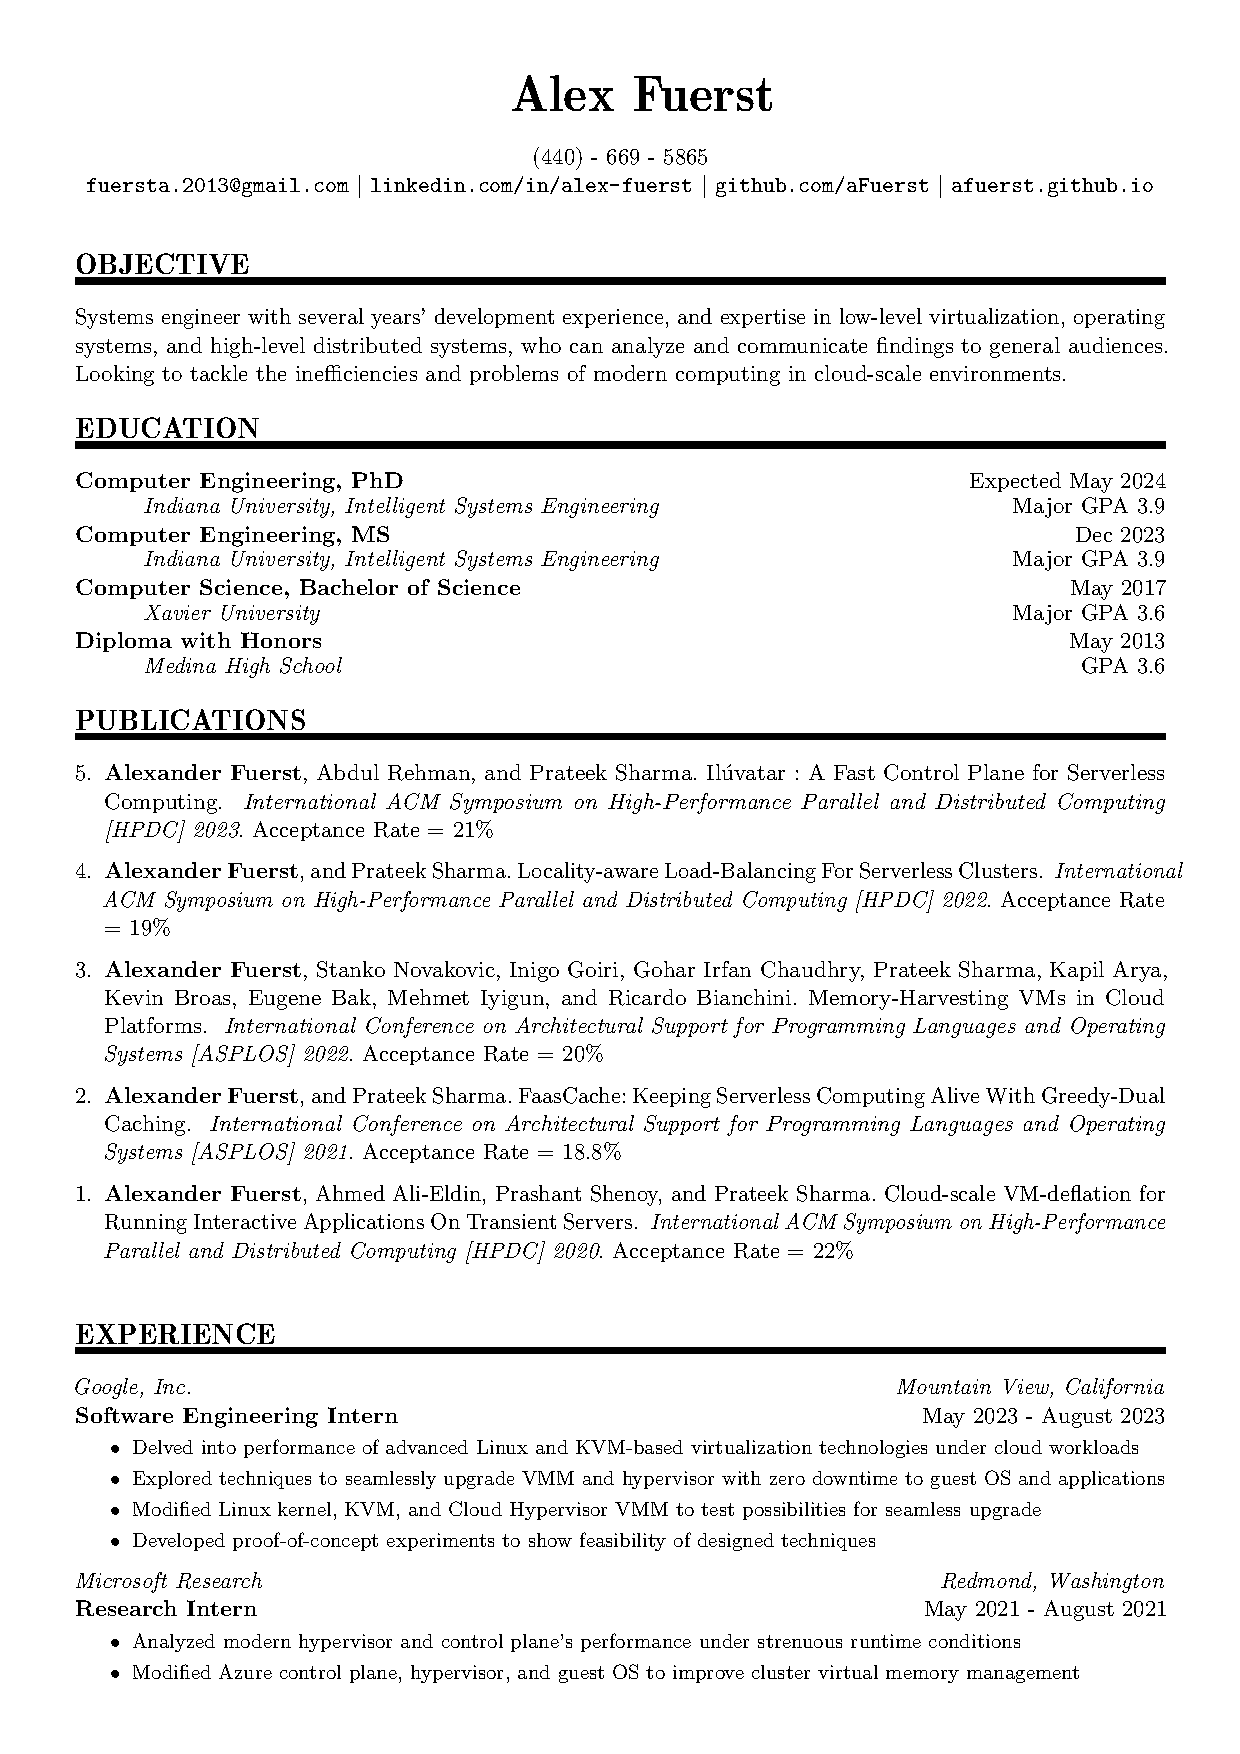
\includepdf[pages=-]{cv/cv.pdf}
